\documentclass[hide notes,intlimits]{beamer}

\mode<presentation>
{
  \usetheme{Singapore}
  \usefonttheme{professionalfonts}
  \setbeamertemplate{blocks}[rounded][shadow=true]
  \setbeamercovered{transparent}
}

% load packages
\usepackage[english]{babel}
\usepackage[latin1]{inputenc}
\usepackage[T1]{fontenc}
\usepackage{lmodern}
\usepackage[multidot]{grffile}
\usepackage{verbatim,empheq}
\usepackage{tikz}
\usetikzlibrary{shapes,arrows,shadows}
\usepackage{animate}

\definecolor{dark red}{HTML}{E41A1C}
\definecolor{dark green}{HTML}{4DAF4A}
\definecolor{dark violet}{HTML}{984EA3}
\definecolor{dark blue}{HTML}{084594}
\definecolor{dark orange}{HTML}{FF7F00}
\definecolor{light blue}{HTML}{377EB8}
\definecolor{light red}{HTML}{FB9A99}
\definecolor{light violet}{HTML}{CAB2D6}

\newcommand{\CC}{\mathbb{C}}
\newcommand{\NN}{\mathbb{N}}
\newcommand{\RR}{\mathbb{R}}
\newcommand{\ZZ}{\mathbb{Z}}

\newcommand{\Kcal}{\mathcal{K}}

\newcommand{\bF}{\mathbf{F}}
\newcommand{\bQ}{\mathbf{Q}}
\newcommand{\bU}{\mathbf{U}}
\newcommand{\bbU}{\bar{\bU}}

\newcommand{\bq}{\mathbf{q}}
\newcommand{\bu}{\mathbf{u}}
\newcommand{\bv}{\mathbf{v}}
\newcommand{\bx}{\mathbf{x}}

\newcommand{\Div}{\nabla\cdot}
\newcommand{\eps}{\epsilon}
\newcommand{\grad}{\nabla}
\newcommand{\lap}{\triangle}
\renewcommand{\bar}{\overline}

\newcommand{\ip}[2]{\ensuremath{\left<#1,#2\right>}}


\newenvironment{transbox}[1][]{%
\begin{tikzpicture}
\node[drop shadow,rounded corners,text width=\textwidth,fill=white, fill opacity=#1,text opacity=1] \bgroup
}{
\egroup;\end{tikzpicture}}


\title[math tools and obstacles in ice sheet models]{Mathematical tools and obstacles \\ in models of ice sheets}

\author[Bueler]{Ed Bueler}

\institute[UAF]{
  \scriptsize Dept of Mathematics and Statistics and Geophysical Institute \\

  University of Alaska Fairbanks \\
  
  \tiny $^{}$ \\
  \tiny supported by NASA grant \# NNX13AM16G
}

\titlegraphic{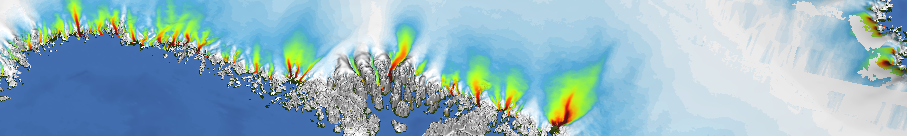
\includegraphics[width=\textwidth]{andycoast.png}}

\setbeamerfont{date}{size=\scriptsize}
\date{}

\AtBeginSection[]
{
  \begin{frame}<beamer>
    \frametitle{Outline}
    %\tableofcontents[currentsection,hideallsubsections]
    \tableofcontents[currentsection]
  \end{frame}
}


\begin{document}

\graphicspath{{figs/}{../commonfigs/}}

\begin{frame}
\vspace{10mm}
  \titlepage
  \begin{center}
  \tiny Denver University \quad 15 May, 2015
  \end{center}
\end{frame}


\section[intro to ice sheets]{I. an introduction to ice sheet flow for non-glaciologists}

\begin{frame}{ice in glaciers is a viscous fluid}
\begin{columns}
\begin{column}{0.65\textwidth}
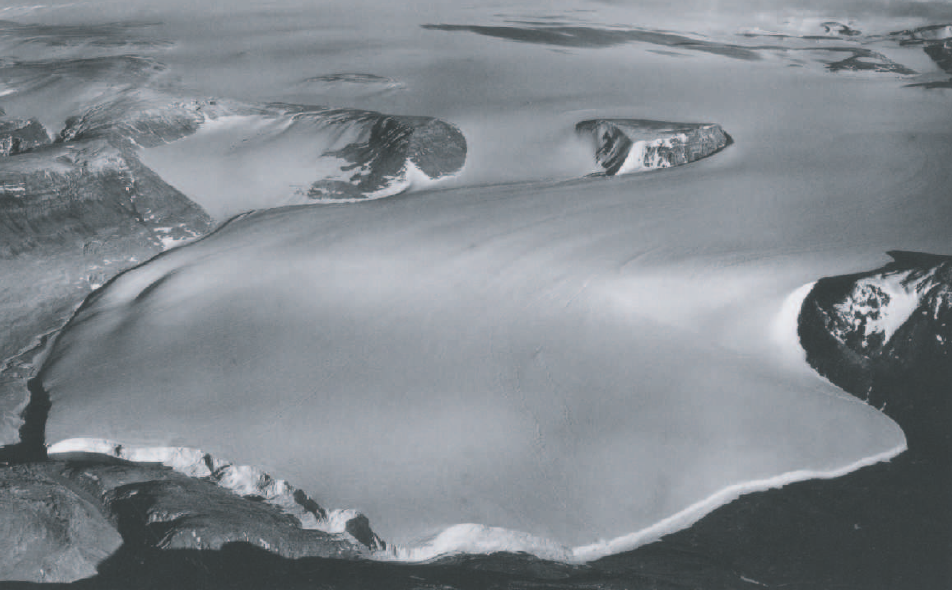
\includegraphics[width=1.0\textwidth]{polaris}
\end{column}
\begin{column}{0.35\textwidth}
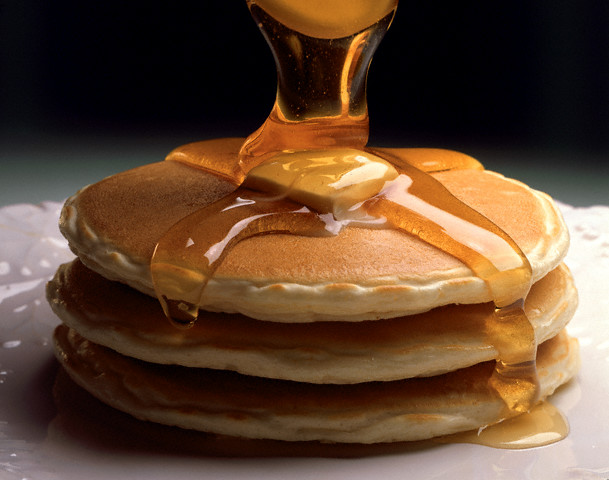
\includegraphics[width=1.0\textwidth]{pancakes}
\end{column}
\end{columns}

\bigskip\bigskip
\begin{itemize}
\item \dots at least: glaciers are viscous flows at larger scales
\item glaciers are free-surface flows (with no surface tension)
\item \emph{usage}: ``ice sheets'' $=$ big, continent-scale glaciers
\end{itemize}
\end{frame}


\begin{frame}{ice in glaciers is a viscous fluid}

\begin{itemize}
\item primary variables: velocity $\mathbf{u}(\bx,t)$ and pressure $p(\bx,t)$
\item also: $\rho$ is density, $\mathbf{g}$ is gravity, $\nu$ is viscosity
\item if the glacier fluid were ``typical'' like the ocean we would model with Navier-Stokes equations:
\begin{align*}
\nabla \cdot \mathbf{u} &= 0 &&\text{\emph{incompressibility}} \\
\rho \left(\mathbf{u}_t + \mathbf{u}\cdot\nabla \mathbf{u}\right) &= -\nabla p + \nu \nabla^2 \mathbf{u} + \rho \mathbf{g} &&\text{\emph{stress balance}}
\end{align*}
\item but ice is not typical!
\item e.g.~not in ice sheet flow models:
  \begin{itemize}
  \item[$\circ$] turbulence
  \item[$\circ$] coriolis force
  \item[$\circ$] convection
  \end{itemize}
\end{itemize}
\end{frame}


\begin{frame}{ice is a slow, shear-thinning viscous fluid}

\begin{itemize}
\item glacier ice is
  \begin{enumerate}
  \item ``slow''\footnote{$Fr\approx 10^{-15}$.  Regarding coriolis: $Fr/Ro \approx 10^{-8}$.}:
    $$\rho \left(\mathbf{u}_t + \mathbf{u}\cdot\nabla \mathbf{u}\right) \approx 0 \qquad \iff \qquad \begin{pmatrix} \text{forces of inertia} \\ \text{are negligible} \end{pmatrix}$$
  \item non-Newtonian shear-thinning\footnote{blood is also shear-thinning \\ \hspace{5mm} corn starch in water is shear-thickening}:
    \begin{itemize}
    \item viscosity $\nu$ is not constant
    \item $\nu$ decreases as fluid is sheared
    \end{itemize}
  \end{enumerate}
\end{itemize}
\end{frame}


\begin{frame}{the standard model}

\begin{itemize}
\item slow flows are called ``Stokes flows''
\item notation:
  \begin{itemize}
  \item[$\circ$] $\tau_{ij}$ is deviatoric stress tensor
  \item[$\circ$] $\mathbf{D}u_{ij}$ is strain rate tensor
  \end{itemize}
\smallskip
\item the standard ice flow model is power-law Stokes:
\begin{align*}
\nabla \cdot \mathbf{u} &= 0 &&\text{\emph{incompressibility}} \\
0 &= - \nabla p + \nabla \cdot \tau_{ij} + \rho \mathbf{g} &&\text{\emph{slow stress balance}} \\
\mathbf{D}u_{ij} &= A \left|\tau_{ij}\right|^{n-1} \tau_{ij} &&\text{\emph{Glen flow law}}
\end{align*}
\item $1.8 < n < 4.0$ ?  \quad \alert{when in doubt: $n=3$}
\medskip
\item $A>0$ is ``ice softness''
   \begin{itemize}
   \item $A$ varies strongly with temperature, but I'll ignore that here
   \end{itemize}
\end{itemize}
\end{frame}


\begin{frame}{model design (because ice is a slow fluid)}

\begin{itemize}
\item ice sheet modeling is a bit like atmosphere flow modeling or weather prediction, but \dots
\item in a Stokes flow, the geometry, boundary stress, and viscosity determine velocity field and pressure, so \dots
\item therefore a time-stepping ice sheet model recomputes the velocity field when needed, without requiring velocity from a previous time-step\footnote{to be a weatherman you've got to know which way the wind blows \dots but not to be a glaciologist}
\end{itemize}
\end{frame}


\begin{frame}{sheets versus streams versus shelves}

\begin{columns}
\begin{column}{0.35\textwidth}
\small
\begin{itemize}
\small
\item non-sliding portions of ice sheets flow by shear deformation
\item ice streams slide too
\item ``ice shelves'' are floating thick ice \dots all sliding
\item ice shelves flow by extension not shear
\item but: sliding ignored for today
\end{itemize}
\end{column}

\begin{column}{0.65\textwidth}
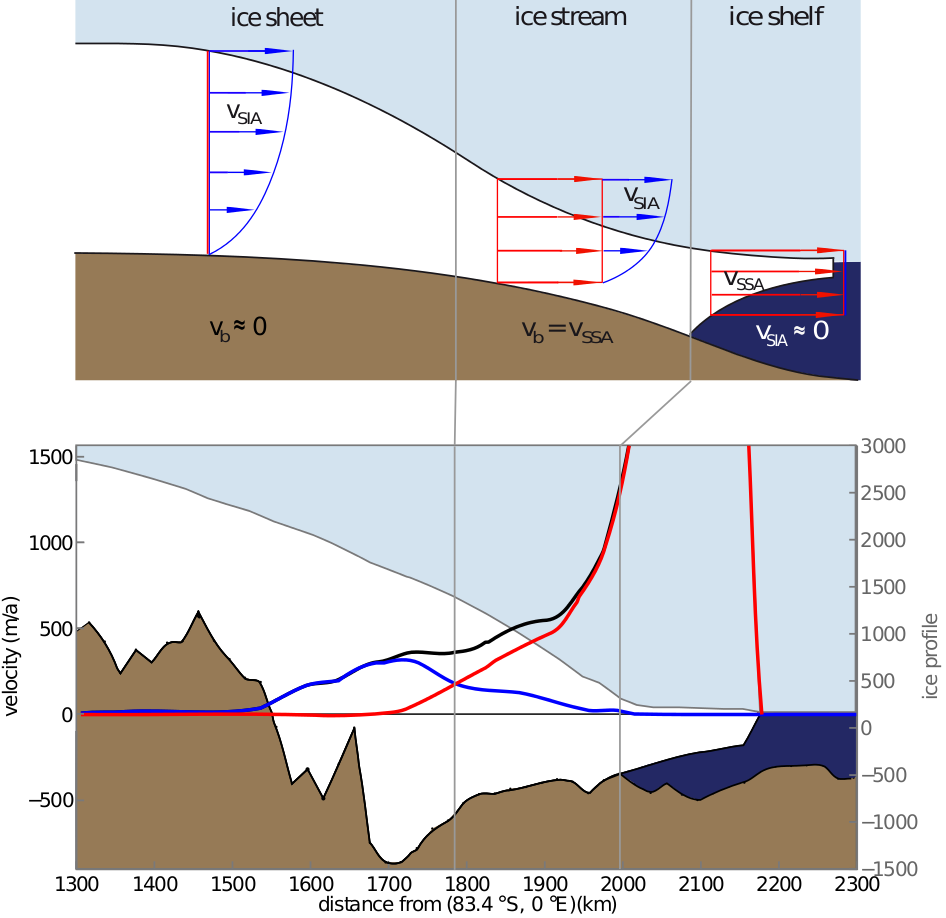
\includegraphics[width=\textwidth]{siassacartoon-lambert}

\begin{center}
\vspace{-0.18in}
\tiny [Lambert glacier and Amery ice shelf, Antarctic]
\end{center}
\end{column}
\end{columns}
\end{frame}


\begin{frame}{ice sheets are shallow}

\begin{itemize}
\item cross-section of Greenland ice sheet at $71^\circ$ N
\small
  \begin{itemize}
  \item[$\circ$] {\color{dark green}{green}} and {\color{dark blue}{blue}}: usual vertically-exaggerated version
  \end{itemize}
  \begin{center}
    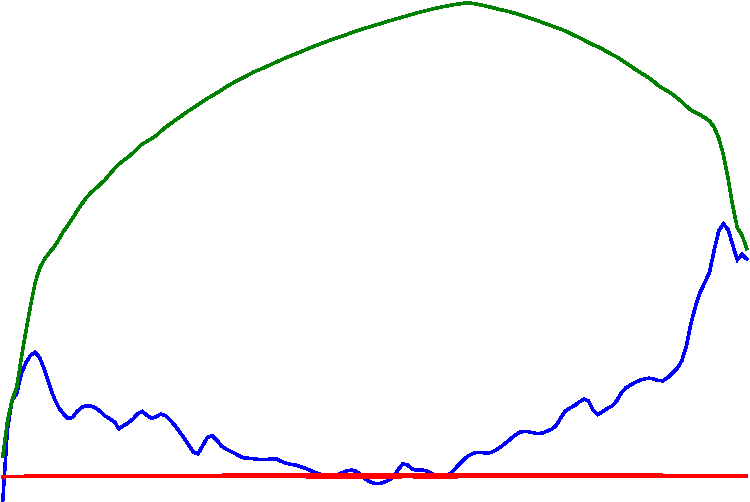
\includegraphics[width=0.5\textwidth]{newgreentrans}
  \end{center}
\normalsize
\item in {\color{dark red}{red}}: a view without this vertical exaggeration
\item \emph{thus}: 
  \begin{itemize}
  \item[$\circ$] most simulations use shallow limits of Stokes
  \item[$\circ$] \scriptsize technical: high aspect-ratio elements bad in non-shallow solvers
  \end{itemize}
\end{itemize}
\end{frame}


\begin{frame}
  \frametitle{first big picture: ice sheets store past climates}
Greenland layers movie from NASA, January 2015
\end{frame}


\begin{frame}
  \frametitle{second big picture: ice sheets affect sea level}
\medskip
\small
\begin{itemize}
\item \emph{mass and energy inputs}: (1) snow adds, (2) sun heats, (3) ocean heats, (4) earth heats
\item \emph{mass outputs}: (1) surface meltwater, (2) basal meltwater, (3) ice discharge
\end{itemize}
\begin{center}
  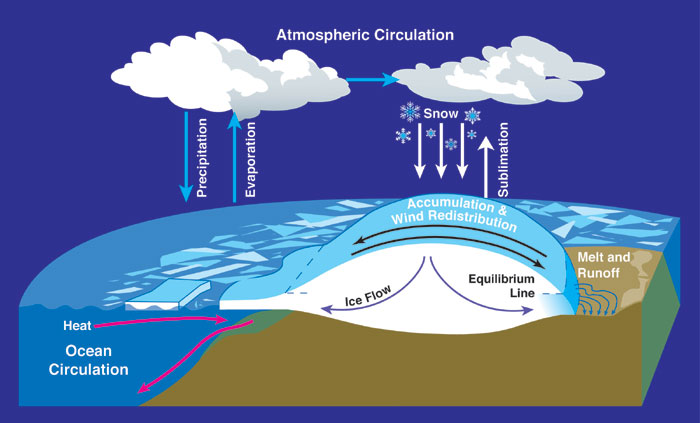
\includegraphics[width=0.75\textwidth]{mass-bal-atmos}
  %\tiny (figure from IceSAT brochure)
\end{center}
\end{frame}


\begin{frame}{summary so far}
\begin{itemize}
\item ice sheets have five outstanding properties as viscous flows:
  \begin{enumerate}
  \item \alert{free surface}
  \item \alert{shallow}
  \item \alert{slow}
  \item \alert{shear-thinning}
  \item \alert{sliding (``contact slip'')}
  \end{enumerate}
\item remainder of my talk will address applied-mathematical questions for models which capture
  \begin{itemize}
  \item[part II] properties 1, 2, 3, 4 but not 5
  \item[part III] \emph{any} time-dependent model which has properties 1 and 2
  \end{itemize}
\end{itemize}
\end{frame}


\section[shallow ice well-posed?]{II. is the shallow ice problem well-posed and approximate-able?}


\begin{frame}
  \frametitle{shallow ice approximation (SIA)}

\begin{itemize}
\item SIA = ``lubrication'' approximation of Stokes model
\item good approximation when:
  \begin{itemize}
  \item[$\circ$] sliding is small or zero
  \item[$\circ$] bedrock slope is modest
  \end{itemize}
\item derive SIA equations by scaling Stokes using shallowness:
  \begin{itemize}
  \item[$\circ$] $[h]$ is a typical thickness scale
  \item[$\circ$] $[x]$ is a typical width scale
  \item[$\circ$] small parameter is $\eps = [h] / [x]$
  \end{itemize}
\end{itemize}
\end{frame}


\begin{frame}
  \frametitle{SIA: velocity}
 
\begin{itemize}
\item $b(x,y)$ is bedrock elevation (data)
\item $s(x,y,t)$ is ice surface elevation (unknown)
\item let $p=n+1>2$
\item assume: no sliding and isothermal
\item horizontal ice velocity is given by: 
  $${\bf U}  =  - \frac{p}{p+1} \Gamma \left[ (s-b)^p - (s - z)^p  \right] 
|\nabla s |^{p-2} \nabla s$$
where $\Gamma > 0$ combines gravity, ice density, ice softness
\end{itemize}
\end{frame}


\begin{frame}
  \frametitle{SIA plus mass conservation in steady state}

\begin{itemize}
\item $a(x,y)$ is snowfall minus melt rate (data)
  \begin{itemize}
  \item[$\circ$] a.k.a.~``surface mass balance''
  \end{itemize}
\item mass conservation in steady state: 
  $$\Div \left(  \int_b^s {\bf U}\, dz \right)  =  a$$
\item shallow ice approximation + (steady) mass conservation:
  $$-\Div \left(\Gamma (s-b)^{p+1} | \nabla s |^{p-2} \nabla s\right) =  a$$
  \begin{itemize}
  \vspace{-0.2in}
  \item[$\circ$] this is ``the SIA equation'' for ice sheet geometry
  \item[$\circ$] like Poisson equation $-\Div (D \grad u) = f$
  \item[$\circ$] $p$-Laplace-ish \dots but coefficient $(s-b)^{p+1} \to 0$ at margins
  \end{itemize}
\item equation above is simplest model for turning data of problem ($b$ and $a$) into ice sheet geometry and velocity ($s$ and $U$)
\end{itemize}
\end{frame}


\begin{frame}{time-dependent SIA}

\begin{itemize}
\item time-dependent SIA equation
  $$\frac{\partial s}{\partial t} + \Div \left(\Gamma (s-b)^{p+1} | \nabla s |^{p-2} \nabla s\right) = a$$
\end{itemize}

\begin{columns}
\begin{column}{0.4\textwidth}
\scriptsize
the Halfar (1983) similarity solution:
  \begin{itemize}
  \scriptsize
  \item[$\circ$] an exact $b=0,a=0$ solution with $t\to 0^+$ limit a delta function
  \item[$\circ$] compare Barenblatt solution of porous medium equation
  \item[$\circ$] movie frames from $t=4$ months to $t = 10^6$ years, equally-spaced in \emph{exponential} time
  \end{itemize}
\end{column}

\begin{column}{0.65\textwidth}
\vspace{-0.25in}
\begin{center}
\animategraphics[autoplay,loop,height=5.2cm]{4}{../commonfigs/animhalfar/halfar}{0}{26}
\end{center}
\end{column}
\end{columns}
\end{frame}


\begin{frame}
  \frametitle{SIA: an analogy}
\begin{columns}
\begin{column}{0.4\textwidth}
\begin{itemize}
\item ice sheet surface \\ $\sim$ \alert{membrane}
\item bedrock $\sim$ \alert{obstacle}
\end{itemize}
\begin{center}
\vspace{-2mm}
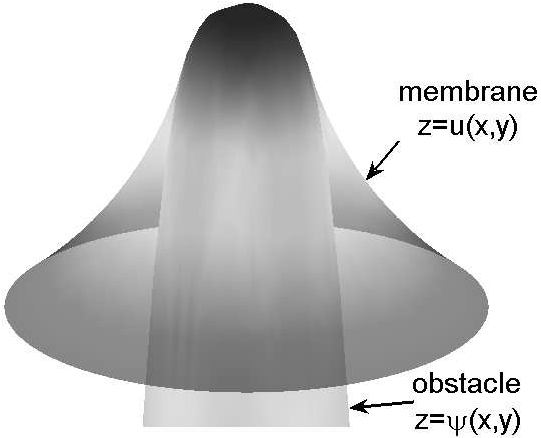
\includegraphics[width=\textwidth]{classicalobs}
\begin{itemize}
\item classical Laplacian obstacle problem:
   $$\lap u = 0 \quad \& \quad u\ge \psi$$
\end{itemize}
\end{center}
\end{column}
\begin{column}{0.55\textwidth}
\begin{center}
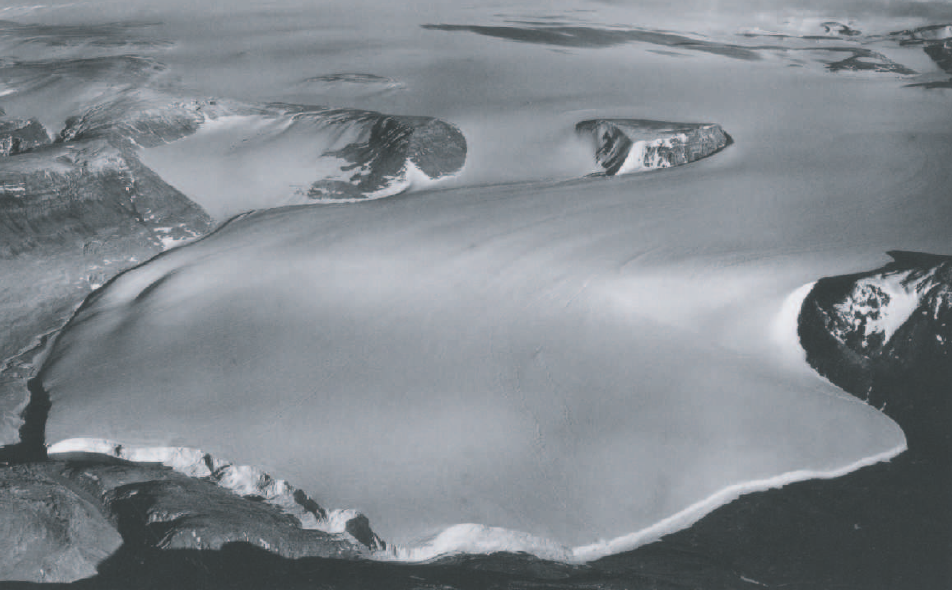
\includegraphics[width=0.95\textwidth]{polaris} \\
\vspace{10mm}
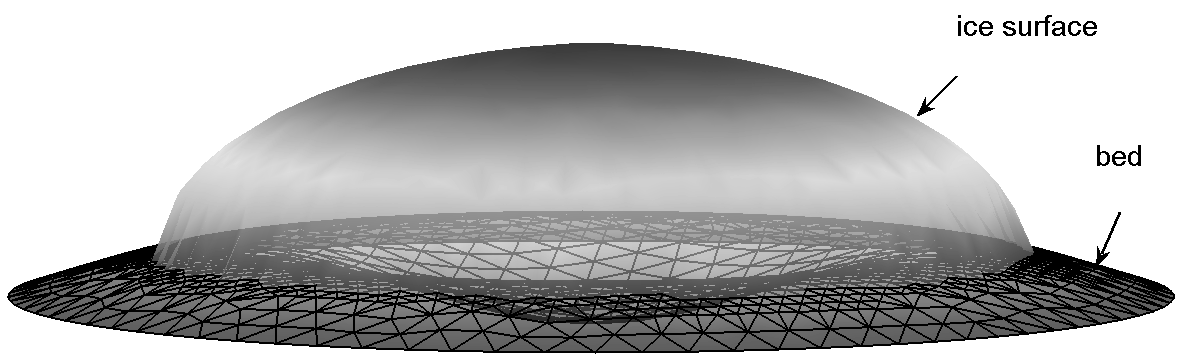
\includegraphics[width=1.05\textwidth]{capnonflatobs}
\end{center}
\end{column}
\end{columns}
\end{frame}


\begin{frame}
  \frametitle{SIA equation is constrained} 
\begin{itemize}
\item $H=s-b$ is ice thickness
\item thickness is a nonnegative quantity!
\item steady state equation ``strong form''
  $$-\Div \left(\Gamma H^{p+1} |\nabla s|^{p-2} \nabla s  \right) =  a$$
applies only where
  $$s>b \qquad \iff \qquad H > 0$$
\end{itemize}
\end{frame}


\begin{frame}{weak formulation by variational inequality} 
\begin{itemize}
\item define convex admissible set
  $$\Kcal := \{\eta : \eta^{2p/(p-1)} \in W^{1,p}_0 (\Omega) \,\text{and}\, \eta \ge 0\}$$
over larger domain $\Omega \subset \RR^2$
\item multiply strong form by $\eta-H$ where $\eta\in \Kcal$, and integrate by parts thoughtfully
\end{itemize}
\begin{block}{definition} 
$H \in \Kcal$ solves the \emph{steady shallow ice sheet problem} if
  $$\int_{\Omega}  \Gamma H^{p+1} |\grad s|^{p-2} \grad s \cdot \grad(\eta - H)  
\ge \int_{\Omega} a (\eta - H)$$
for all $\eta \in \Kcal$
\end{block}
\end{frame}


\begin{frame}{ideas contained in weak formulation} 
\begin{itemize}
\item weak form
  $$\int_{\Omega}  \Gamma H^{p+1} |\grad s|^{p-2} \grad s \cdot \grad(\eta - H)  
\ge \int_{\Omega} a (\eta - H)$$
implies strong form
  $$-\Div \left(\Gamma H^{p+1} |\nabla s|^{p-2} \nabla s  \right) =  a$$
where $H>0$
\item where $H=0$, weak form implies $a \le 0$
\item if $b=0$ the weak form is equivalent to a constrained minimization problem, but for general bed this is not so
\end{itemize}
\end{frame}


\begin{frame}{on well-posedness (Jouvet-Bueler 2012)} 
\begin{block}{theorem.}
if $b=0$ then the variational inequality is equivalent to
  $$\min \, J[u] = \int_{\Omega} \frac{\Gamma}{p} |\grad u|^p - a u$$
over $\eta = u^{(p-1)/(2p)} \in \Kcal$, and this problem is well-posed (existence, uniqueness, stability w.r.t.~data $a$)
\end{block}
\begin{block}{theorem.}
in general case ($b\ne 0$) there exists a solution
\end{block}
\begin{proof}[proof]
fixed-point theorem, of course
\end{proof}
\end{frame}


\begin{frame}{an interesting quality of this variational inequality} 
\begin{itemize}
\item every glaciologist believes this about steady climates:
\begin{center}
 if $a>0$ on $R$ then $H>0$ on $R$
\end{center}
that is:
\begin{center}
 if it snows more than it melts then you get a glacier
\end{center}
\end{itemize}
\begin{columns}
\begin{column}{0.6\textwidth}
\begin{itemize}
\small
\item uniformly-elliptic variational inequalities, e.g.~the classical obstacle problem,
\begin{align*}
\int_{\Omega}  \nabla u \cdot \nabla (v - u)  \ge  \int_{\Omega} f (v - u),
\end{align*}
for all $v\ge \psi$, do \emph{not} have the analogous property
\end{itemize}
\end{column}
\begin{column}{0.35\textwidth}
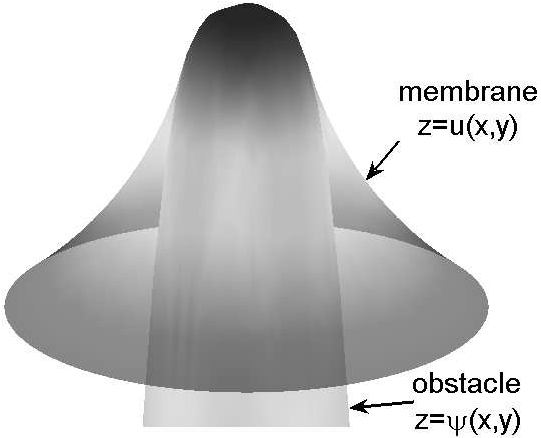
\includegraphics[width=0.95\textwidth]{classicalobs}
\end{column}
\end{columns}
\end{frame}


\begin{frame}{another weak form} 
\begin{itemize}
\item the variational inequality has abstract form
  $$- \ip{\bq(H,\grad H)}{\grad(\eta - H)} \ge \ip{a}{\eta-H} \qquad \forall \eta \in \Kcal$$
where $\bq=\int_b^s {\bf U}\, dz=-\Gamma H^{p+1} |\grad s|^{p-2} \grad s$ is the ``flux''
\item a standard localization argument gives
  $$F \ge 0 \quad \text{ and } \quad H\,F = 0$$
where $F = \Div \bq - a$
\begin{block}{definition.}
for $f:\RR^m \to \RR^m$, we say $x^* \in \RR^m$ solves the \emph{nonlinear complementarity problem} (NCP) if
  $$x^* \ge 0  \quad \text{ and } \quad f(x^*)\ge 0 \quad \text{ and } \quad x^*\,f(x^*)=0$$
\end{block}
\item scalable Newton solvers are available for NCPs
\end{itemize}
\end{frame}


\begin{frame}{example computation: steady Greenland ice sheet}
\begin{columns}
\begin{column}{0.6\textwidth}
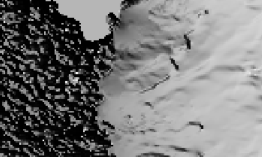
\includegraphics[width=1.05\textwidth]{insetinset}
\vfill
\begin{itemize}
\small
\item data is $b(x,y)$ and $a(x,y)$
\item 900 m grid on $1500\times 2600$ km domain
\item NCP solved on 192 processors
  \begin{itemize}
  \scriptsize
  \item[$\circ$] reduced-space Newton solver (PETSc)
  \item[$\circ$] double continuation by
    \begin{itemize}
    \scriptsize
    \item[$\circ$] diffusivity regularization
    \item[$\circ$] bed smoothing
    \end{itemize}
  \end{itemize}
\end{itemize}
\end{column}
\begin{column}{0.4\textwidth}
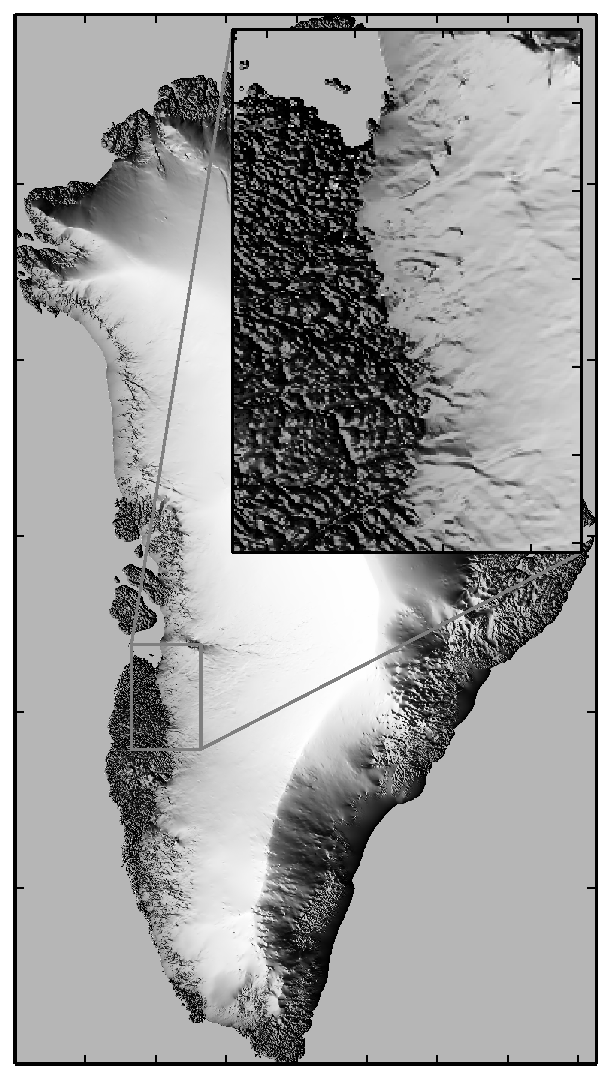
\includegraphics[height=0.85\textheight]{grnwinset}

\tiny Bueler (submitted)
\end{column}
\end{columns}
\end{frame}


\begin{frame}{Greenland velocity from a better model}
\begin{center}
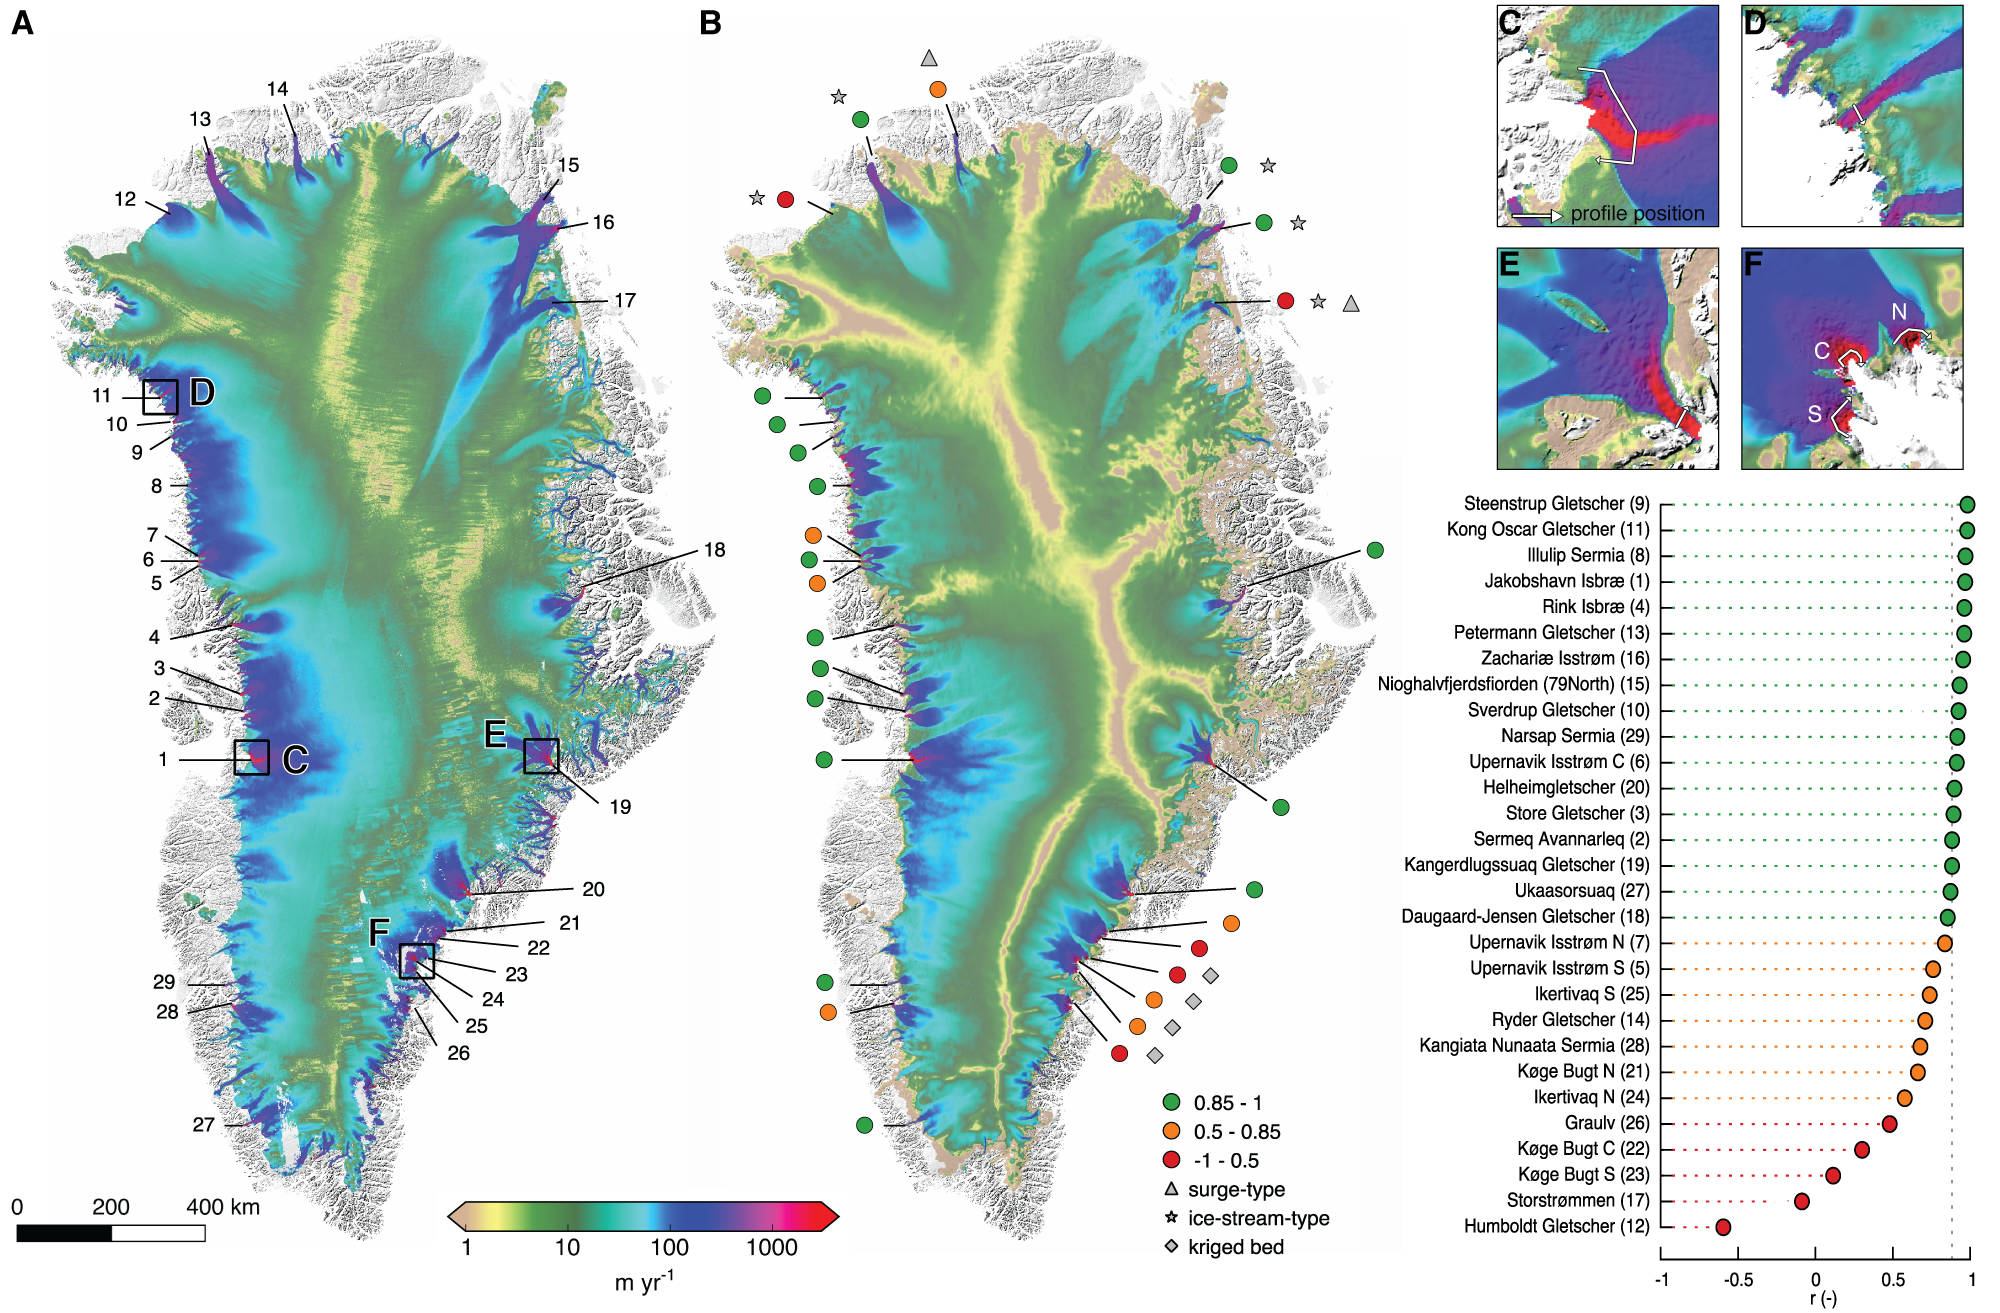
\includegraphics[width=1.0\textwidth]{greenland-overview}
\end{center}

\vspace{-5mm}
\tiny Aschwanden et al (submitted); model is the Parallel Ice Sheet Model (\texttt{pism-docs.org})
\end{frame}


\section[conservation w free boundaries?]{III. can thin-layer free-boundary models exactly conserve?}

\begin{frame}
  \frametitle{thin layers in a ``climate''}
\begin{center}
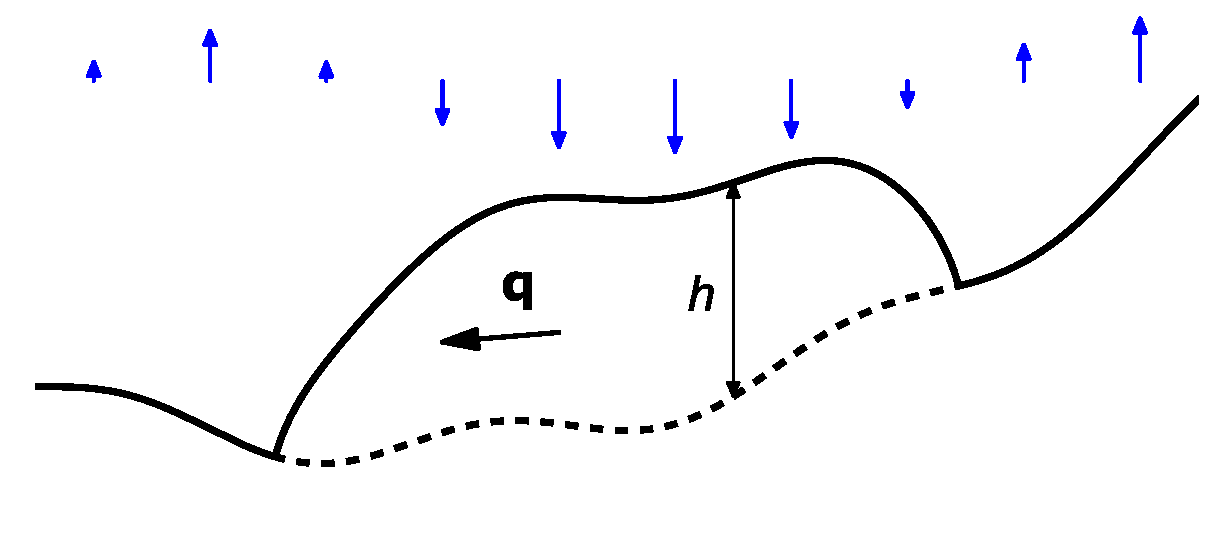
\includegraphics[width=0.65\textwidth,keepaspectratio=true]{cartoon-wclimate}
\end{center}
\vspace{-6mm}
\begin{itemize}
\item abstract problem (strong form)
  \begin{equation}
  h_t + \Div \bq = {\color{blue} f} \tag{$\ast$}
  \end{equation}
on $\Omega \subset \RR^2$, where $\bq=\bq(\grad h, h, x, t)$ and ${\color{blue} f}={\color{blue} f}(h,x,t)$
\item $h$ is layer thickness, $\bq$ is flux, and ${\color{blue} f}$ is source or ``climate''
\item PDE ($\ast$) can be parabolic or hyperbolic \dots
  \begin{itemize}
  \item[$\circ$] but it only applies where $h>0$
  \end{itemize}
\item ``$h\ge 0$'' needs to be a constraint
  \begin{itemize}
  \item[$\circ$] generates free boundary somewhere in region where ${\color{blue} f} < 0$
  \end{itemize}
\end{itemize}
\end{frame}


\begin{frame}
  \frametitle{examples}
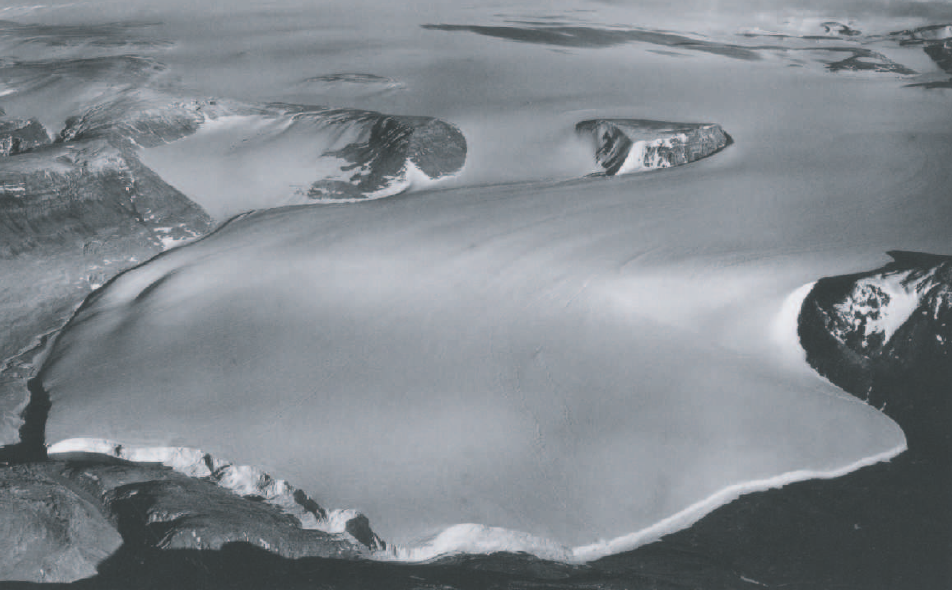
\includegraphics[width=0.4\textwidth,keepaspectratio=true]{polaris}
\hfill
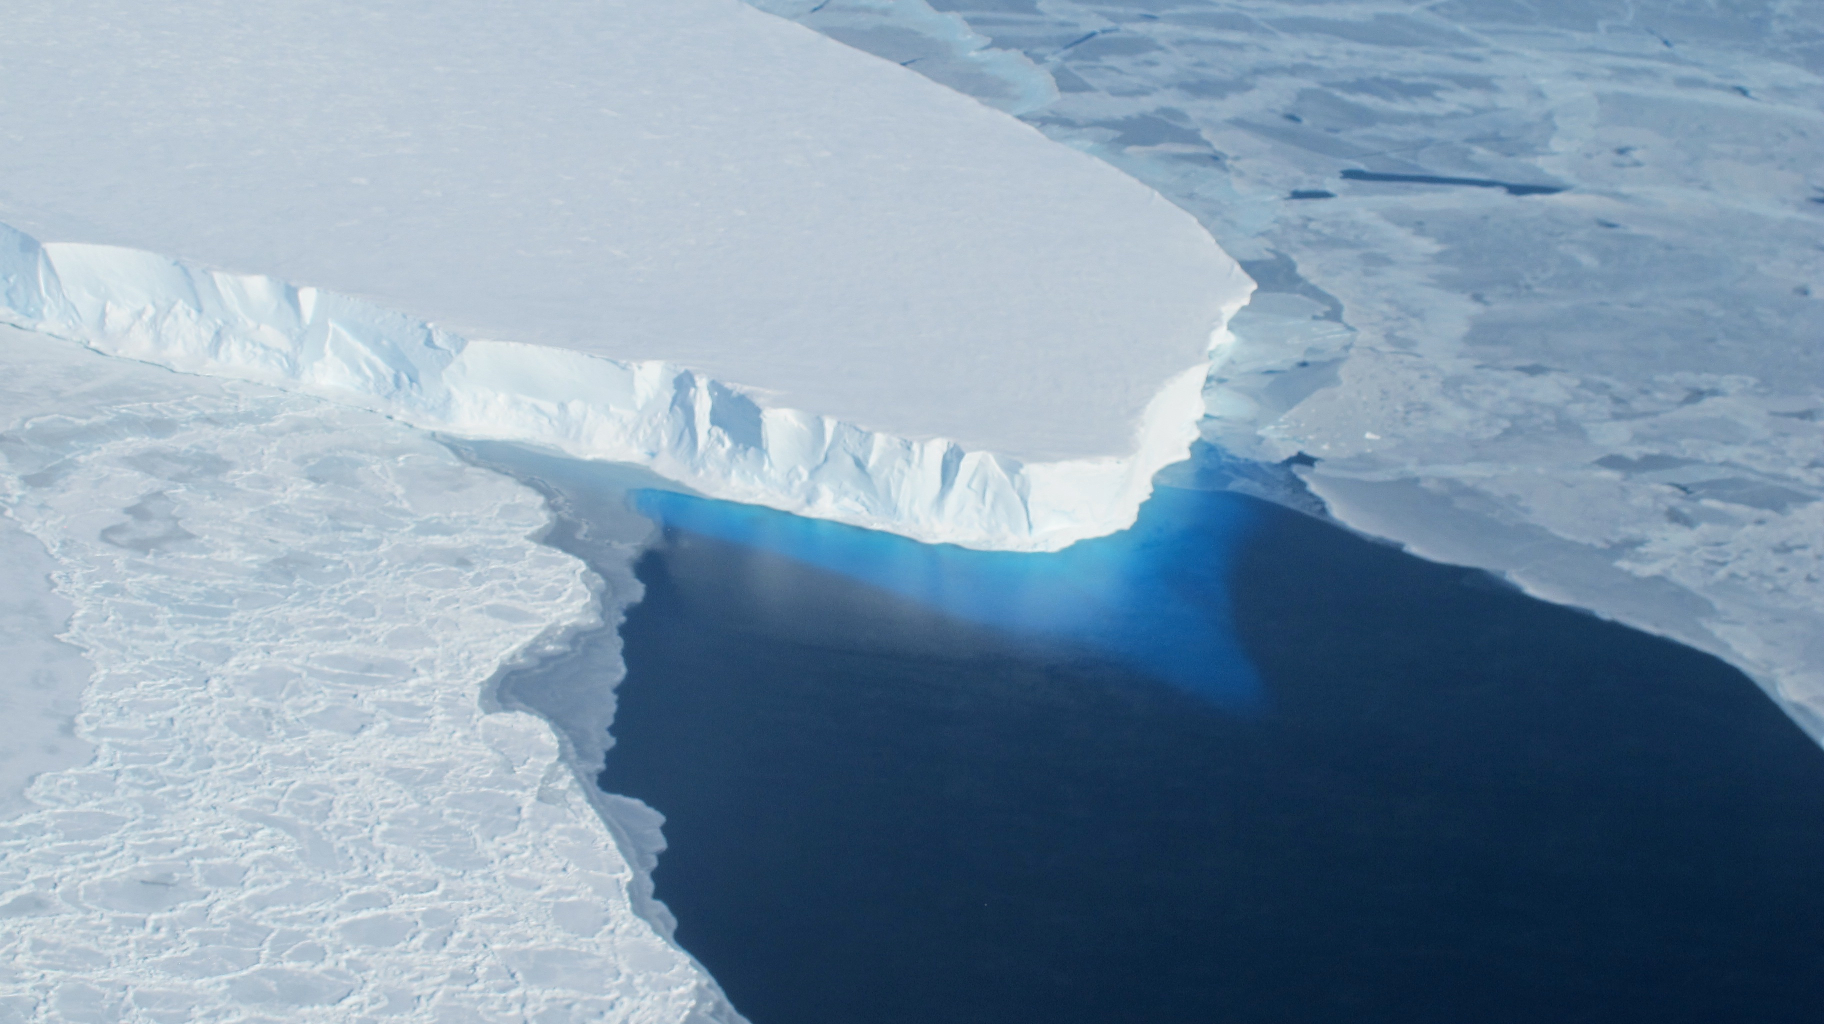
\includegraphics[width=0.45\textwidth,keepaspectratio=true]{supp4rignot-small}

\small glaciers \hfill ice shelves \& sea ice
\medskip

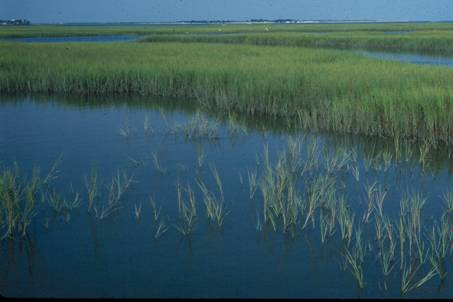
\includegraphics[width=0.41\textwidth,keepaspectratio=true]{marsh-water}
\hfill
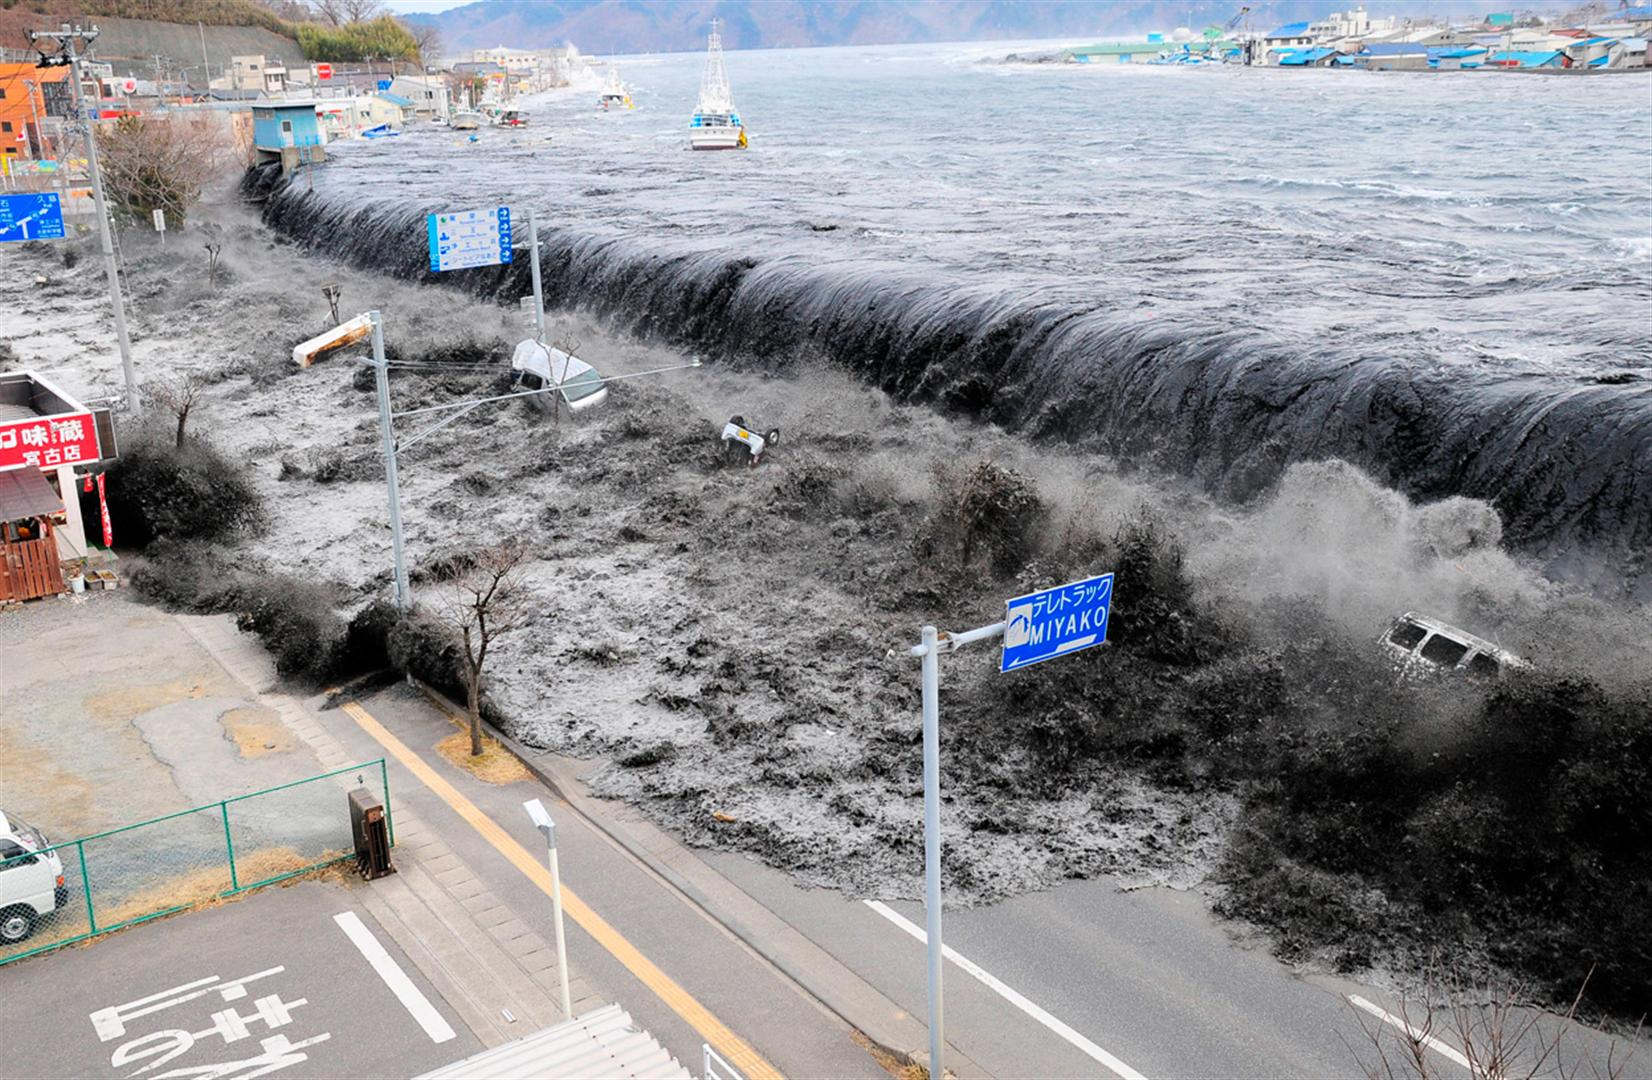
\includegraphics[width=0.42\textwidth,keepaspectratio=true]{tsunami-sendai}

\small tidewater marsh \hfill tsunami inundation

\scriptsize and sea-level rise, surface hydrology, subglacial hydrology, \dots
\end{frame}


\begin{frame}
  \frametitle{discrete time}
\begin{itemize}
\item numerical models for this equation \emph{must} discretize time:
  $$(\ast) \longrightarrow \frac{h_n - h_{n-1}}{\Delta t} + \Div \bQ_n = F_n$$
  \begin{itemize}
  \item[$\circ$] in minimal sense: semi-discretize ($\ast$) = ``$u_t + \Div \bq = f$'' in time
  \end{itemize}
\item this might be by backward Euler, trapezoid, RK, \dots
\item but remember constraint: $h_n \ge 0$
\item questions:
  \begin{itemize}
  \item[$\circ$] are implicit time-steps well-posed?
    \begin{itemize}
    \item[$\triangleright$] explicit time steps are always well-posed here, but cause severe stability time-step restrictions
    \end{itemize}
  \item[$\circ$] FIXME
  \end{itemize}
\end{itemize}
\begin{center}
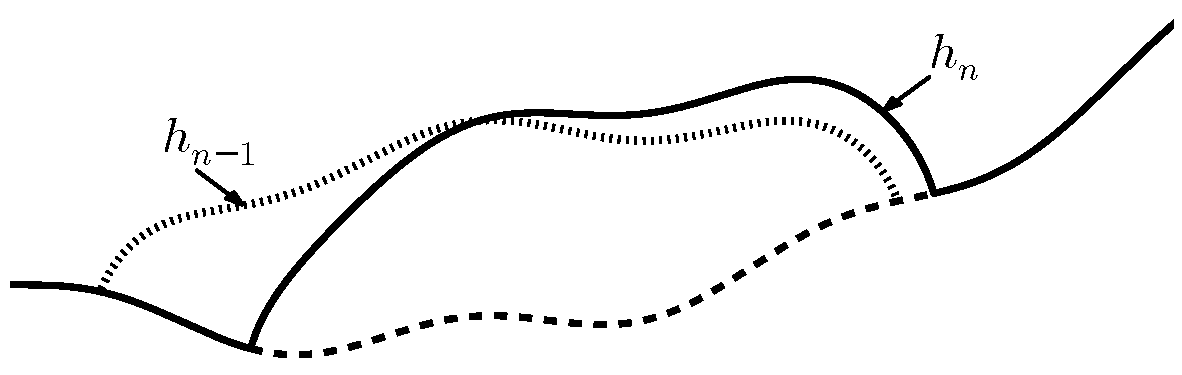
\includegraphics[width=0.85\textwidth,keepaspectratio=true]{cartoon-sets-crop}
\end{center}
\end{frame}


\begin{frame}
  \frametitle{weak form of an implicit time step}
FIXME
\end{frame}


\begin{frame}
  \frametitle{solution sets}
FIXME

\begin{center}
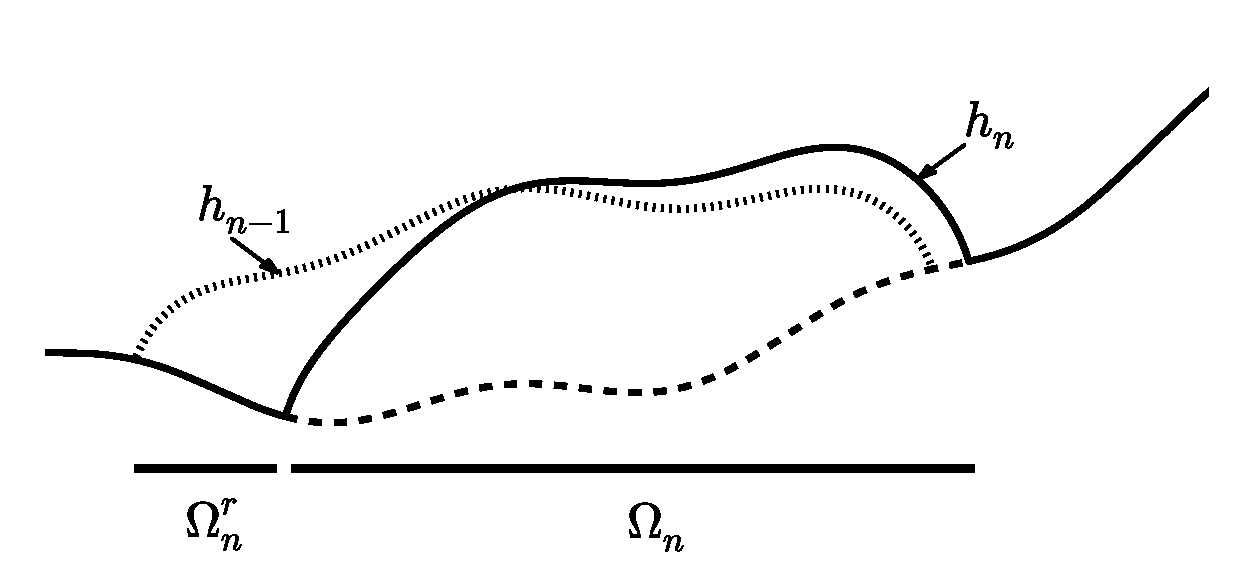
\includegraphics[width=0.85\textwidth,keepaspectratio=true]{cartoon-sets}
\end{center}
\end{frame}


\section*{conclusion}

\begin{frame}
  \frametitle{conclusion}

\begin{itemize}
\item is shallow ice problem
  \begin{itemize}
  \item[$\circ$] well-posed? \qquad \alert{probably}
  \item[$\circ$] approximate-able? \qquad \alert{yes}
     \begin{itemize}
     \item[$\triangleright$] but how fast and reliably?
     \end{itemize}
  \end{itemize}
\item can thin-layer free-boundary problems
  \begin{itemize}
  \item[$\circ$] be solved by implicit time-stepping? \qquad \alert{yes}
  \item[$\circ$] be exactly discrete conserving? \qquad \alert{no}
     \begin{itemize}
     \item[$\triangleright$] but error can be quantified
     \end{itemize}
  \end{itemize}
\end{itemize}
\end{frame}

\end{document}
